\documentclass[journal, a4paper]{IEEEtran}
\usepackage{graphicx}   
\usepackage{url}
\usepackage{amsmath} 
\usepackage[utf8]{inputenc}
\usepackage{graphicx} 
\usepackage{float}
\usepackage{wrapfig}
\usepackage{pgfplots}
\usepackage{tikz}
\usepackage{cite}
\usetikzlibrary{positioning}
\DeclareMathAlphabet{\mathpzc}{OT1}{pzc}{m}{it}


\tikzset{%
   neuron missing/.style={
    draw=none, 
    scale=4,
    text height=0.333cm,
    execute at begin node=\color{black}$\vdots$
  },
}

\pgfplotsset{width = 5cm, compat=1.13}
\pgfplotsset{every axis/.append style={
    axis x line=middle,    % put the x axis in the middle
    axis y line=middle,    % put the y axis in the middle
    axis line style={<->}, % arrows on the axis
    },
    cmhplot/.style={color=blue,mark=none,line width=1pt,<->},
}

\begin{document}
	\title{Multimedia processing using machine learning}
	\author{Jakub Bielawa, Paweł Cejrowski, Łukasz Dawidowski, Łukasz Myśliński, Agata Radys}
	\markboth{Gdansk University of Technology, ETI department}{}
	\maketitle

\begin{abstract}
Some abstract
\end{abstract}

\section{Introduction}
The field of digital audio processing is an interesting topic, broadly investigated in scientific research. Problems such as music genre or instrument classification have been sucessfully solved in the past with the use of traditional machine learning methods. In this paper we analyse the results of "ISMIS 2011 Contest: Music Information Retrieval/Music Genres", and try to improve the results achieved in that challange. 
\section{Theory}
\subsection{Neural networks}
\subsubsection{Fully connected neural network}
A fully connected neural network (FCNN) is such a neural network in which each neuron is connected to every neuron in the previous layer and each connection has its own weight. \par This is a general purpose connection pattern and makes no assumptions about the features in the input data to recognize. This type of network is very expensive in terms of memory (weights) and computations (connections).
\begin{figure}[H]
\centering
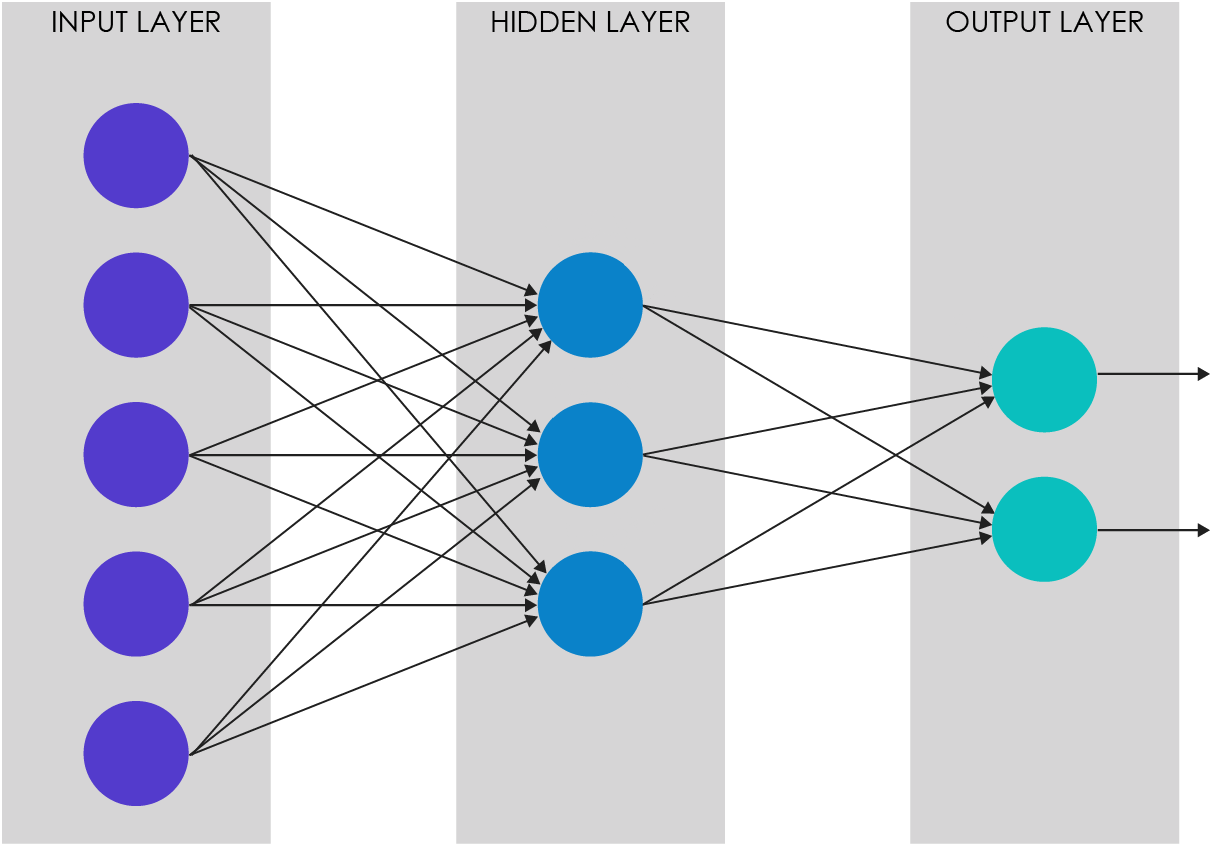
\includegraphics[width=250px]{pictures/fcnn.png}
\caption{Fully connected neural network}
\end{figure}

\subsubsection{Convolutional neural network}
Convolutional neural network (CNN) is a type of feed-forward artificial neural network, which means that connections between the neurons do not form a cycle. Information in the network moves only forward so the given signal goes through the neuron once.
\par CNN includes a convolutional layer and usually few other hidden layers. Each neuron is connected only to a small region of the previous layer called receptive field. Receptive fields of different neurons are overlapping with other neuron's fields so that together they are covering the whole input.
\par CNN are used for image processing because while using convolution they can recognize edges of an object on the image.
\begin{figure}[H]
\centering
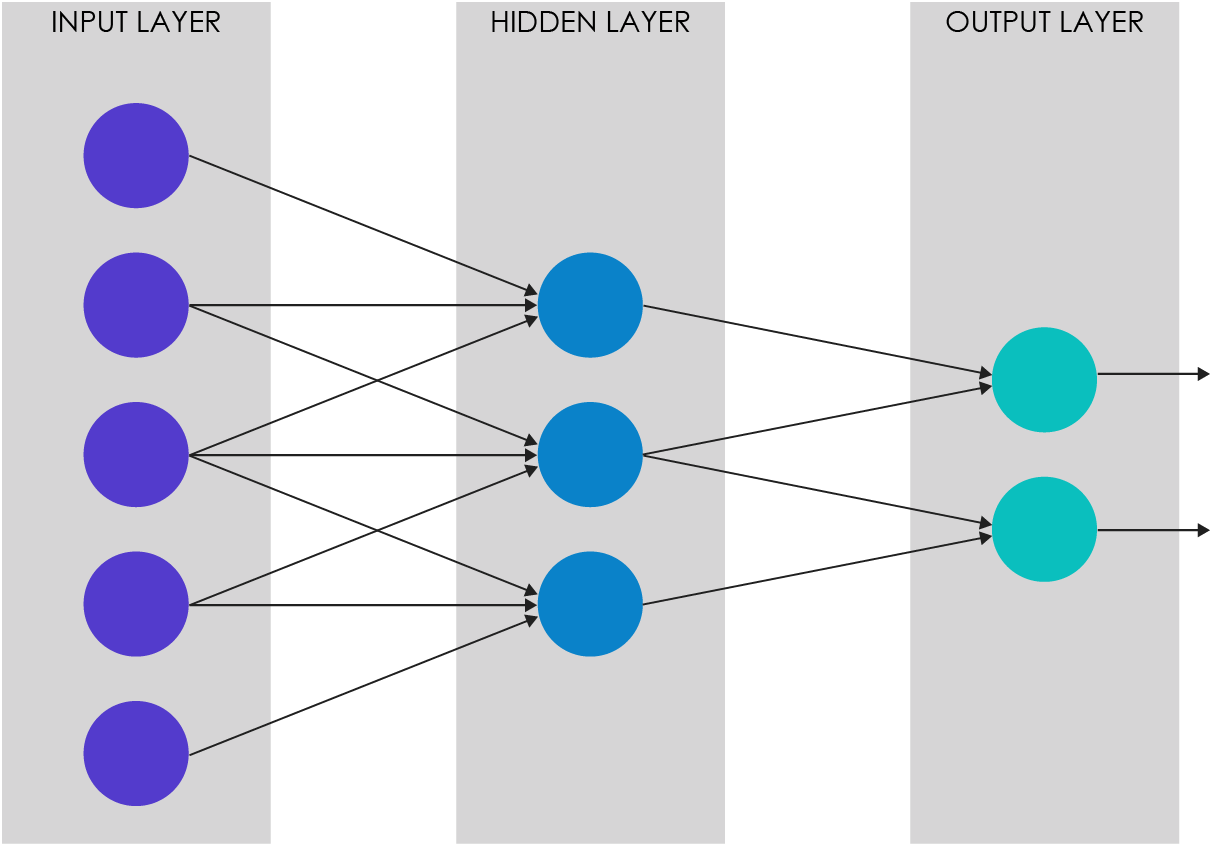
\includegraphics[width=250px]{pictures/cnn.png}
\caption{Convolutional neural network}
\end{figure}

\subsubsection{Recurrent neural network}
In recurrent neural network (RNN) connections between the neurons form a directed cycle. It means that RNN can use its internal memory to learn  sequences of inputs. The same set of weights is applied recursively to the structure.
\par RNN are used for text or speech recognition.
\begin{figure}[H]
\centering
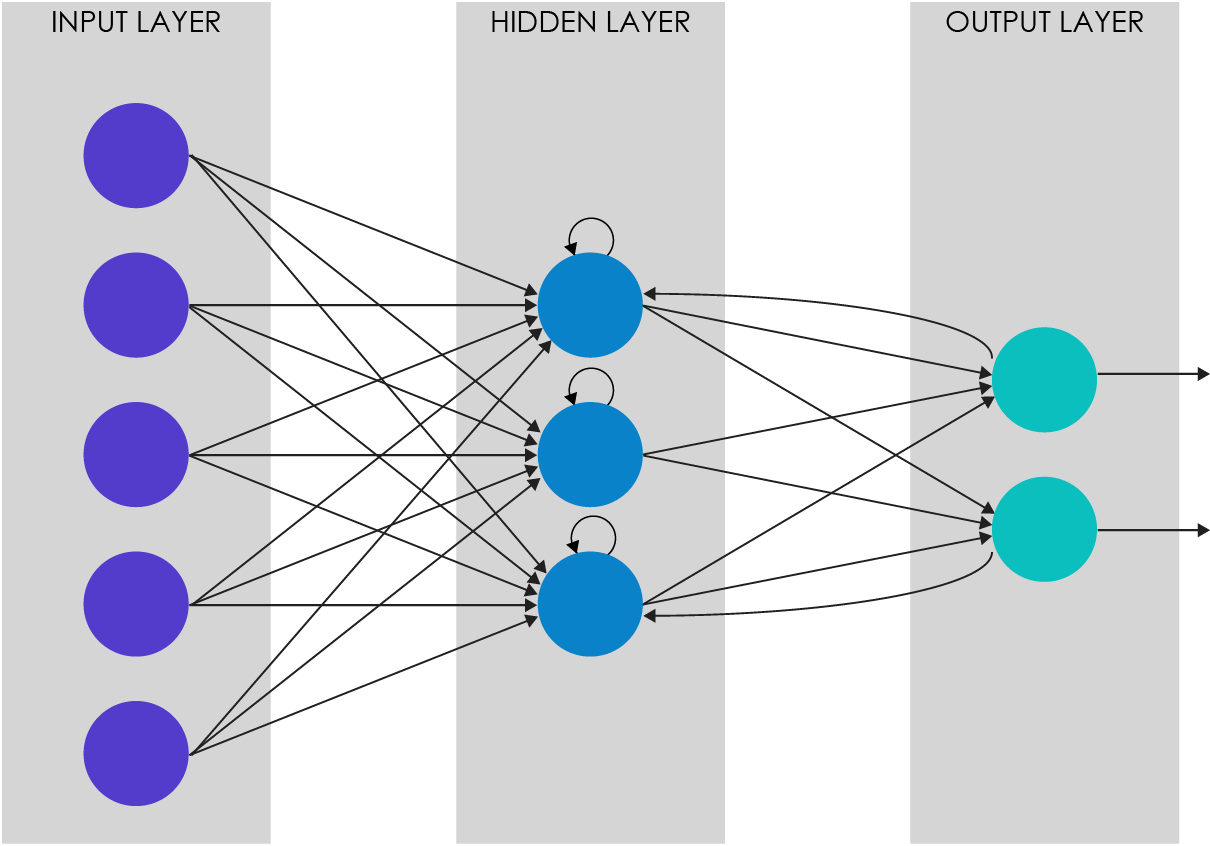
\includegraphics[width=250px]{pictures/rnn.png}
\caption{Convolutional neural network}
\end{figure}

\subsection{Activation function}
The activation function defines the output of considered neuron with given input. There are many functions that can be used as an activation function in artificial neural networks. The most popular are:
\subsubsection{Linear}
\begin{center}
$ f(x)=ax + b $ \\ $ a,b \in R $ \\~\\
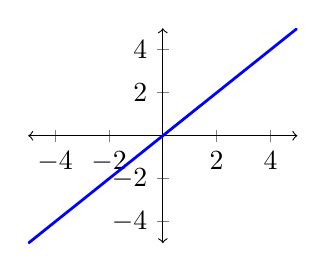
\begin{tikzpicture}
	\begin{axis}
		\addplot[cmhplot,-]{x};
	\end{axis}
\end{tikzpicture}
\end{center}

\subsubsection{Rectified Linear Unit (ReLU)}
\[
f(x)=
\left\{
\begin{array}{ll}
      0 ,& x < 0 \\
      x ,& x\geq 0 \\
\end{array} 
\right. \]
\begin{center}
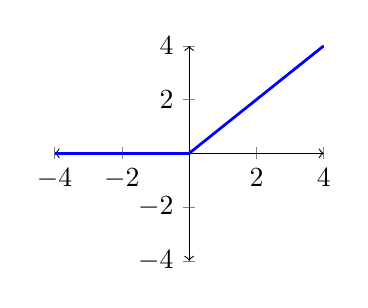
\begin{tikzpicture}
    \begin{axis}[
            xmin=-4,xmax=4,
            ymin=-4,ymax=4,
        ]
        \addplot[cmhplot,-,domain=-4:0]{0};
        \addplot[cmhplot,-,domain=0:4]{x};

    \end{axis}
\end{tikzpicture}
\end{center}

\subsubsection{Sigmoid}
\begin{center}
$f(x) = \frac{1}{1 + e^{-x}}$ \\
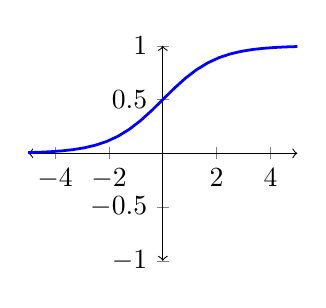
\begin{tikzpicture}
    \begin{axis}[
            xmin=-5,xmax=5,
            ymin=-1,ymax=1,
        ]
        \addplot[cmhplot,-]{1/(1 + e^(-x))};
    \end{axis}
\end{tikzpicture}
\end{center}

\subsubsection{TanH}
\begin{center}
$ f(x)=\tanh(x)=\frac{2}{1+e^{-2x}}-1 $ \\
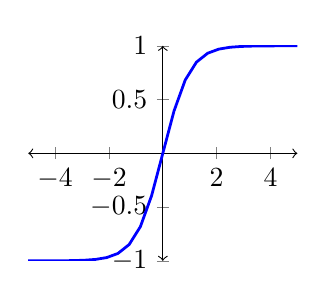
\begin{tikzpicture}
    \begin{axis}[
            xmin=-5,xmax=5,
            ymin=-1,ymax=1,
        ]
        \addplot[cmhplot,-]{2/(1 + e^(-2*x))-1};
    \end{axis}
\end{tikzpicture}
\end{center}

\subsection{Optimization and regularization}
\subsubsection{Dropout}
\subsubsection{Initial weights}
\subsubsection{Learning rate decay}
\subsubsection{Gradient Descent}

\subsection{Features}
An audio track in a digital format is represented by a discrete set of values identifying a sound wave. In order to apply machine learning techniques to a track, identifiers for each track is required. With the use of mathematical transformations like the Fourier transformation and its derivaties a collection of values representing each sample is aquired. In this particular study, the feature extraction process has already been applied. Features represeting each track are listed below.

\begin{enumerate}
\item Temporal Centroid 
\item Spectral Centroid average value 
\item Spectral Centroid variance
\item Audio Spectrum Envelope (ASE) average values in 34 frequency bands
\item ASE average value (averaged for all frequency bands)
\item ASE variance values in 34 frequency bands
\item averaged ASE variance parameters
\item Audio Spectrum Centroid – average and variance values
\item Audio Spectrum Spread – average and variance values
\item Spectral Flatness Measure (SFM) average values for 24 frequency bands
\item SFM average value (averaged for all frequency bands)
\item Spectral Flatness Measure (SFM) variance values for 24 frequency bands
\item averaged SFM variance parameters
\item 20 first mel cepstral coefficients average values 
\item dedicated parameters in time domain based of the analysis of the distribution of the envelope in relation to the rms value.
\end{enumerate}

There parameters sum up to a total of 191 values used to identify track's musical identity. 


\section{Architecture}
As a solution for genre recognition problem, authors propose fully connected 4-hidden-layer neural network built up on TensorFlow framework. Hidden layers consist of $1024$, $1024$, $256$ and $56$ nodes. High-level architecture of the Depp Neural Network is presented in Figure \ref{fig:dnn}. Learning rate decaying is used with parameters as in equation \ref{eq:rate_decay}.
\begin{equation}
learning\ rate = 0.3 \times 0.9^{\frac{step}{500}}
\label{eq:rate_decay}
\end{equation}
Moreover, dropout is used during training after each of the hidden layers on the level of $0.7$, which means that $30\%$ is dropped out. After input layer and $4$ hidden layers ReLU activation function is used, whereas Softmax with cross entropy is used after the output layer. The network is optimized using Gradient Descent algorithm. Initial weights are randomly selected from $\mathcal{N}(0,0.05)$ for hidden layers and $\mathcal{N}(0,0.1)$ for output layer. Initial biases are set to $0$. 

\begin{figure}[H]%
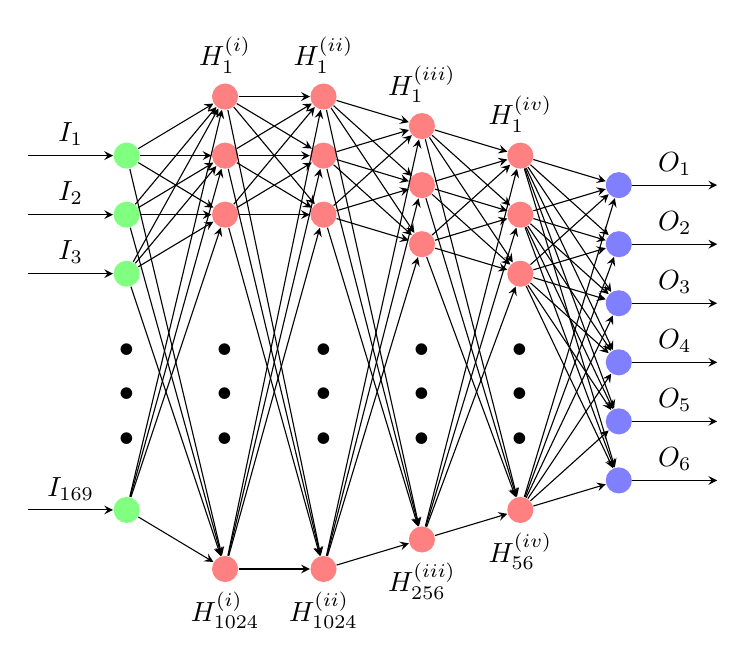
\begin{tikzpicture}[x=1.25cm, y=1.5cm, >=stealth]

\foreach \m/\l [count=\y] in {1,2,3}
{
 \node [circle,fill=green!50,minimum size=0.2cm] (input-\m) at (0,1.25-0.5*\y) {};
}
\foreach \m/\l [count=\y] in {4}
{
 \node [circle,fill=green!50,minimum size=0.2cm ] (input-\m) at (0,-1.25-\y) {};
}
 
 \node [neuron missing]  at (0,-1.25) {};
 

\foreach \m [count=\y] in {1,2,3}
  \node [circle,fill=red!50,minimum size=0.2cm ] (hidden1-\m) at (1,1.75-0.5*\y) {};
  
\foreach \m [count=\y] in {4}
  \node [circle,fill=red!50,minimum size=0.2cm ] (hidden1-\m) at (1,-2.75) {};
  
 \node [neuron missing]  at (1,-1.25) {};



\foreach \m [count=\y] in {1,2,3}
  \node [circle,fill=red!50,minimum size=0.2cm ] (hidden2-\m) at (2,1.75-0.5*\y) {};
  
\foreach \m [count=\y] in {4}
  \node [circle,fill=red!50,minimum size=0.2cm ] (hidden2-\m) at (2,-2.75) {};
  
 \node [neuron missing]  at (2,-1.25) {};



\foreach \m [count=\y] in {1,2,3}
  \node [circle,fill=red!50,minimum size=0.2cm ] (hidden3-\m) at (3,1.5-0.5*\y) {};
  
\foreach \m [count=\y] in {4}
  \node [circle,fill=red!50,minimum size=0.2cm ] (hidden3-\m) at (3,-2.5) {};
  
 \node [neuron missing]  at (3,-1.25) {};



\foreach \m [count=\y] in {1,2,3}
  \node [circle,fill=red!50,minimum size=0.2cm ] (hidden4-\m) at (4,1.25-0.5*\y) {};
  
\foreach \m [count=\y] in {4}
  \node [circle,fill=red!50,minimum size=0.2cm ] (hidden4-\m) at (4,-2.25) {};
  
 \node [neuron missing]  at (4,-1.25) {};



% output layer
\foreach \m [count=\y] in {1}
  \node [circle,fill=blue!50,minimum size=0.2cm ] (output-\m) at (5,1.5-\y) {};
\foreach \m [count=\y] in {2}
  \node [circle,fill=blue!50,minimum size=0.2cm ] (output-\m) at (5,1.0-\y) {};
\foreach \m [count=\y] in {3}
  \node [circle,fill=blue!50,minimum size=0.2cm ] (output-\m) at (5,0.5-\y) {};
\foreach \m [count=\y] in {4}
  \node [circle,fill=blue!50,minimum size=0.2cm ] (output-\m) at (5,0.0-\y) {};
\foreach \m [count=\y] in {5}
  \node [circle,fill=blue!50,minimum size=0.2cm ] (output-\m) at (5,-0.5-\y) {};
\foreach \m [count=\y] in {6}
  \node [circle,fill=blue!50,minimum size=0.2cm ] (output-\m) at (5,-1.0-\y) {};

%%%%%%%%%%%%%%%%%%%%%%%%%%%%%%%%%%%%%%%%%%%%%%%%%%%%%%%%%%%%%%%%%%%%%%%%%%%%%
% labels

\foreach \l [count=\i] in {1,2,3,169}
  \draw [<-] (input-\i) -- ++(-1,0)
    node [above, midway] {$I_{\l}$};

\foreach \l [count=\i] in {1}
  \node [above] at (hidden1-\i.north) {$H^{(i)}_{\l}$};

\foreach \l [count=\i] in {1}
  \node [above] at (hidden2-\i.north) {$H^{(ii)}_{\l}$};

\foreach \l [count=\i] in {1}
  \node [above] at (hidden3-\i.north) {$H^{(iii)}_{\l}$};

\foreach \l [count=\i] in {1}
  \node [above] at (hidden4-\i.north) {$H^{(iv)}_{\l}$};

\foreach \l [count=\i] in {1024}
  \node [below] at (hidden1-4.south) {$H^{(i)}_{\l}$};

\foreach \l [count=\i] in {1024}
  \node [below] at (hidden2-4.south) {$H^{(ii)}_{\l}$};

\foreach \l [count=\i] in {256}
  \node [below] at (hidden3-4.south) {$H^{(iii)}_{\l}$};

\foreach \l [count=\i] in {56}
  \node [below] at (hidden4-4.south) {$H^{(iv)}_{\l}$};



\foreach \l [count=\i] in {1,2,3,4,5,6}
  \draw [->] (output-\i) -- ++(1,0)
    node [above, midway] {$O_{ \l}$};
		
%%%%%%%%%%%%%%%%%%%%%%%%%%%%%%%%%%%%%%%%%%%%%%%%%%%%%%%%%%%%%%%%%%%%%%%%%%%%%
% connections

\foreach \i in {1,...,4}
  \foreach \j in {1,...,4}
    \draw [->] (input-\i) -- (hidden1-\j);

\foreach \i in {1,...,4}
  \foreach \j in {1,...,4}
    \draw [->] (hidden1-\i) -- (hidden2-\j);
\foreach \i in {1,...,4}
  \foreach \j in {1,...,4}
    \draw [->] (hidden2-\i) -- (hidden3-\j);
		\foreach \i in {1,...,4}
  \foreach \j in {1,...,4}
    \draw [->] (hidden3-\i) -- (hidden4-\j);
\foreach \i in {1,...,4}
  \foreach \j in {1,...,6}
    \draw [->] (hidden4-\i) -- (output-\j);

\end{tikzpicture}
\caption{Deep neural network schema}%
\label{fig:dnn}%
\end{figure}


	
\section{Experiments}
\subsubsection{ISMIS Dataset}
 Initially, data from \cite{data} was used. The sample ISMIS dataset provided to the contestants consists of nearly 26000 separate audio tracks from 10 genres. Each track is already processed and represent in the form of audio features. The dataset has been divided into two equally-sized datasets - one for training the network, and one for testing. Solutions, that is the information about the genre of each track has only been provided for the train dataset. Table 1 lists the percentage results of top competitors:
\begin{table}[h]
	\centering
	\caption{ISMIS contestants results}
	\label{my-label}
	\begin{tabular}{|l|l|l|ll}
		\cline{1-3}
		Rank & Team      & Final Result &  &  \\ \cline{1-3}
		1    & domcastro & 0.87507      &  &  \\ \cline{1-3}
		2    & tester    & 0.87270      &  &  \\ \cline{1-3}
		3    & wahoo     & 0.83066      &  &  \\ \cline{1-3}
	\end{tabular}
\end{table}

As we can observe, the best score achieved in the challange is 87.507\% classfication success rate. 
In order to replicate the contest, due to lack of solutions for the entire dataset we have based our reserach solely on the train dataset. The initial 13000 dataset has been divided into two smaller groups, each spanning 6500 tracks. Odd tracks were chosen for the test set, and even tracks for the train set. Furthermore, the dataset order has been randomized to increase scientific accuracy of our study. 

The network has been trained with the train dataset in 3000 steps. After the training, the net has been tested against the test dataset. We were able to achieve an impressive result of 96.4\% classfication success rate, a significant improval over results achieved by the competitors in the study. 

\subsubsection{GZTAN Dataset}
Second round of experiments was focused on data from \cite{gztan}. The GZTAN dataset consists of 1000 audio tracks, each 30 seconds long, divided into 10 genres, represented by 100 tracks each. All tracks are 20050Hz Mono 16-bit audio files in .wav format. Because of this additional work to extract sound characteristics from each track was required. The goal was to replicate the features present in \cite{data} as closely as possible, due to posivite results with such data. 145 distinct descriptors for each audio file were extracted, described in detail in previous sections. \newline
Due to signifant diffrences between descriptor values, normalization was performed. Each descriptor was recalculated with the following formula:
\begin{center}
	$d` = \frac{d - \mu}{\sigma}  $ \\~\\
\end{center}
The network configuration remained unchaged from previous experiment. Suprisingly, a success rate of only 63.66\% was achieved. Dataset reduction was performed to see if less categories would yield better results. 

\begin{table}[h]
	\centering
	\caption{GZTAN success rate \% vs category count}
	\label{my-label}
	\begin{tabular}{|l|l|l|l|l|l|}
		\cline{1-6}
		Category count & 6 & 7 &  8 & 9 & 10  \\ \cline{1-6}
		Dataset size   & 600 & 700 & 800 & 900 & 1000 \\ \cline{1-6}
		Success rate   & 75.06\% & 67.78\% & 64.48 \% & 64.08\% & 63.66\% \\ \cline{1-6}
	\end{tabular}
\end{table}

As presented in Table II, the performance of the neural network did not improve to satisfactory results along with the dataset reduction.

\subsubsection{Summary} Further investigation did not provide any more useful information, as to why the performance differs so much between datasets. While the authors of the \cite{gztan} admit, that the data has been collected from random sources over the years, low coherence of the dataset should not affect the neural net performance so vastly. 





\section{Conclusions}

Results are partially satisfying. While a very good result on an established dataset from \cite{data} was obtained, an attempt to process raw sound database, such as in \cite{gztan} has failed to deliver good results. In order to decisively establish the legitimacy of the networks architecture further research is required. Validating against more datasets is desirable.

\bibliography{bibliography}{}
\bibliographystyle{plain}
\end{document}
